\documentclass[11pt]{article}
\usepackage{amsmath,amssymb}
\usepackage{tikz}
\usetikzlibrary{arrows.meta,positioning}
\begin{document}
\section*{T017 / T020 Dependency Map}
\begin{center}
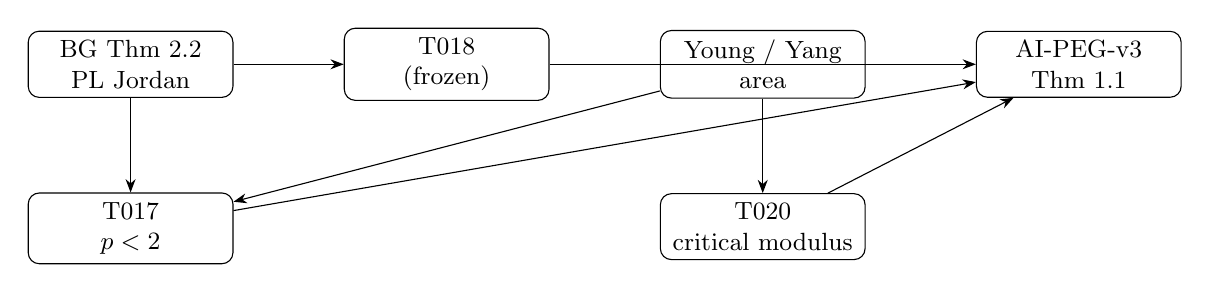
\begin{tikzpicture}[
  node distance=1.1cm and 1.4cm,
  box/.style={draw, rounded corners, align=center, minimum width=2.6cm, font=\small}
]
  \node[box] (bg) {BG Thm 2.2\\PL Jordan};
  \node[box, right=of bg] (t018) {T018\\(frozen)};
  \node[box, right=of t018] (young) {Young / Yang\\area};
  \node[box, right=of young] (ai) {AI-PEG-v3\\Thm 1.1};
  \node[box, below=1.2cm of bg] (t017) {T017\\$p<2$};
  \node[box, below=1.2cm of young] (t020) {T020\\critical modulus};
  \draw[-{Stealth}] (bg) -- (t018);
  \draw[-{Stealth}] (t018) -- (ai);
  \draw[-{Stealth}] (bg) -- (t017);
  \draw[-{Stealth}] (young) -- (t017);
  \draw[-{Stealth}] (young) -- (t020);
  \draw[-{Stealth}] (t017) -- (ai);
  \draw[-{Stealth}] (t020) -- (ai);
\end{tikzpicture}
\end{center}
\end{document}
